\documentclass[conference]{IEEEtran}
\IEEEoverridecommandlockouts

\usepackage{cite}
\usepackage{amsmath}
\usepackage[T1]{fontenc}
\usepackage{newtxtext,newtxmath}
\usepackage[scaled=0.88]{beramono}
\usepackage{graphicx}
\usepackage{textcomp}
\usepackage{xcolor}
\usepackage{booktabs}
\usepackage{multirow}
\usepackage{siunitx}
\usepackage{tikz}
\usetikzlibrary{arrows.meta,positioning,fit,backgrounds,calc,shapes.geometric}
\usepackage{pgfplots}
\pgfplotsset{compat=1.18}
\usepackage[hidelinks]{hyperref}

% Values that still have to be measured on the live AWS deployment render in red.
\newcommand{\needsdata}[1]{\textcolor{red}{\textbf{[#1]}}}

% Starts a new row of author blocks (3 authors on the first row, 2 on the second).
\makeatletter
\newcommand{\linebreakand}{%
  \end{@IEEEauthorhalign}
  \hfill\mbox{}\par
  \mbox{}\hfill\begin{@IEEEauthorhalign}
}
\makeatother

\begin{document}

\title{StreamForge: A Cost-Aware, Event-Driven Architecture for Cloud Video Transcoding and Delivery with Scale-to-Zero Workers}

\author{
\IEEEauthorblockN{Kartika Dhonde}
\IEEEauthorblockA{\textit{Department of Computer Engineering} \\
\textit{Mukesh Patel School of Technology}\\
\textit{Management and Engineering}\\
\textit{NMIMS University}\\
Mumbai, India \\
kartika.dhonde16@nmims.in}
\and
\IEEEauthorblockN{Kshitij Jhalak}
\IEEEauthorblockA{\textit{Department of Computer Engineering} \\
\textit{Mukesh Patel School of Technology}\\
\textit{Management and Engineering}\\
\textit{NMIMS University}\\
Mumbai, India \\
kshitij.jhalak90@nmims.in}
\and
\IEEEauthorblockN{Shlok Doshi}
\IEEEauthorblockA{\textit{Department of Computer Engineering} \\
\textit{Mukesh Patel School of Technology}\\
\textit{Management and Engineering}\\
\textit{NMIMS University}\\
Mumbai, India \\
shlok.doshi49@nmims.in}
\linebreakand
\IEEEauthorblockN{Samar Kamat}
\IEEEauthorblockA{\textit{Department of Computer Engineering} \\
\textit{Mukesh Patel School of Technology}\\
\textit{Management and Engineering}\\
\textit{NMIMS University}\\
Mumbai, India \\
samar.kamat06@nmims.in}
\and
\IEEEauthorblockN{Rama Varshney}
\IEEEauthorblockA{\textit{Department of Computer Engineering} \\
\textit{Mukesh Patel School of Technology}\\
\textit{Management and Engineering}\\
\textit{NMIMS University}\\
Mumbai, India \\
rama.varshney@nmims.edu}
}

\maketitle

\begin{abstract}
Video processing workloads are bursty and compute-heavy, which makes them expensive to host on always-on servers and awkward to run on function-as-a-service platforms with short execution limits. This paper presents StreamForge, an open-source platform on Amazon Web Services (AWS) that ingests user uploads, transcodes them into 720p and 480p H.264 renditions with a JPEG thumbnail, and delivers them through a content delivery network. Browsers upload directly to object storage through presigned URLs, so the control-plane API never carries media bytes. Storage events feed a message queue whose depth drives a containerized FFmpeg worker fleet on Fargate Spot that scales between zero and three tasks. A dead-letter queue bounds the cost of malformed inputs. The entire stack (53 Terraform resource blocks) is declared as code and is deployed by a GitHub Actions pipeline that uses OpenID Connect federation instead of stored credentials, blocks images with fixable critical vulnerabilities, and detects automatic rollbacks by the ECS deployment circuit breaker. We benchmark the production worker image under a 1-vCPU, 2-GB resource limit matching the deployed task size and find that a 1080p clip takes about 1.53~s of processing per second of video, that the two renditions together are about 86\% smaller than the 8~Mb/s source, and that the 1-vCPU size is inefficient: a 2-vCPU limit is 2.6$\times$ faster. We also present a cost model showing that, with no NAT gateway and an idle worker cost of zero, the always-on footprint reduces to one load balancer and one small API task.
\end{abstract}

\begin{IEEEkeywords}
cloud computing, video transcoding, event-driven architecture, serverless containers, autoscaling, infrastructure as code, CI/CD, DevSecOps
\end{IEEEkeywords}

%% ---------------------------------------------------------------------------
\section{Introduction}
Video dominates consumer internet traffic~\cite{cisco_vni}, and nearly every application that accepts user video must convert uploads into a small set of standard renditions before it can stream them. Transcoding is CPU-bound, takes time proportional to clip duration, and arrives in bursts. Running it on dedicated virtual machines means paying for idle capacity between bursts. Running it on function-as-a-service (FaaS) platforms avoids idle cost~\cite{jonas2019cloud} but runs into per-invocation duration, memory and ephemeral-storage limits~\cite{aws_lambda_quotas}, and full-length transcodes do not fit them without restructuring the encoder~\cite{fouladi2017excamera,ao2018sprocket}.

There is a second, less discussed cost problem. Reference cloud architectures often place compute in private subnets behind managed NAT gateways, provision databases, and run several CDN distributions. For student, prototype and small-team budgets, these fixed costs can exceed the variable cost of the workload itself.

This paper describes StreamForge, a video upload, transcoding and streaming platform designed to keep fixed cost low while retaining the operational properties expected of production systems: elastic processing, bounded failure cost, least-privilege access, reproducible infrastructure, and automated, verifiable deployment. Its contributions are:
\begin{enumerate}
  \item An event-driven architecture in which media bytes never pass through the API tier, with worker capacity derived from queue depth and scaled to zero when idle (Section~\ref{sec:design}).
  \item A failure model built on at-least-once queue delivery, idempotent output keys and a dead-letter queue, with an explicit analysis of Spot interruption and duplicate delivery (Sections~\ref{sec:design-queue} and~\ref{sec:discussion}).
  \item A fully declarative deployment and a delivery pipeline that uses keyless OIDC federation, image vulnerability gating and circuit-breaker rollback detection (Section~\ref{sec:impl}).
  \item A measurement of the production worker image under the deployed resource limits, and a cost model of the fixed and per-job costs (Section~\ref{sec:eval}).
\end{enumerate}
The source code, infrastructure definitions and workflows are publicly available~\cite{streamforge_repo}.

%% ---------------------------------------------------------------------------
\section{Related Work}
\textbf{Serverless video processing.} ExCamera~\cite{fouladi2017excamera} showed that splitting a video into small chunks and encoding them across thousands of short-lived functions can cut latency by orders of magnitude, at the cost of a custom encoder that passes state between chunks. Sprocket~\cite{ao2018sprocket} generalized this into a serverless video processing framework with a pipeline abstraction. Both target latency for long videos. StreamForge targets cost and operational simplicity for short user-generated clips: it runs an unmodified FFmpeg~\cite{ffmpeg} per job inside a container, which avoids FaaS duration limits without changing the encoder.

\textbf{Encoding and streaming.} H.264/AVC~\cite{wiegand2003overview} remains the most widely decodable codec. Production services choose encoding ladders per title~\cite{netflix_pertitle} and stream them with adaptive protocols such as MPEG-DASH~\cite{stockhammer2011dash}. StreamForge uses a fixed two-rung ladder with progressive MP4 download and manual resolution selection. Section~\ref{sec:conclusion} discusses moving to segmented adaptive streaming.

\textbf{Cluster management and delivery practice.} Container orchestration grew out of large-scale cluster managers~\cite{burns2016borg}. StreamForge uses a managed serverless container service, so it does not operate a cluster. Its pipeline follows continuous delivery practice~\cite{humble2010continuous}, infrastructure-as-code principles~\cite{morris2020iac}, and container security guidance~\cite{nist800190}. Its rollback behavior applies the circuit-breaker pattern~\cite{nygard2018release} at the deployment level.

%% ---------------------------------------------------------------------------
\section{System Design}\label{sec:design}

\begin{figure*}[t]
\centering
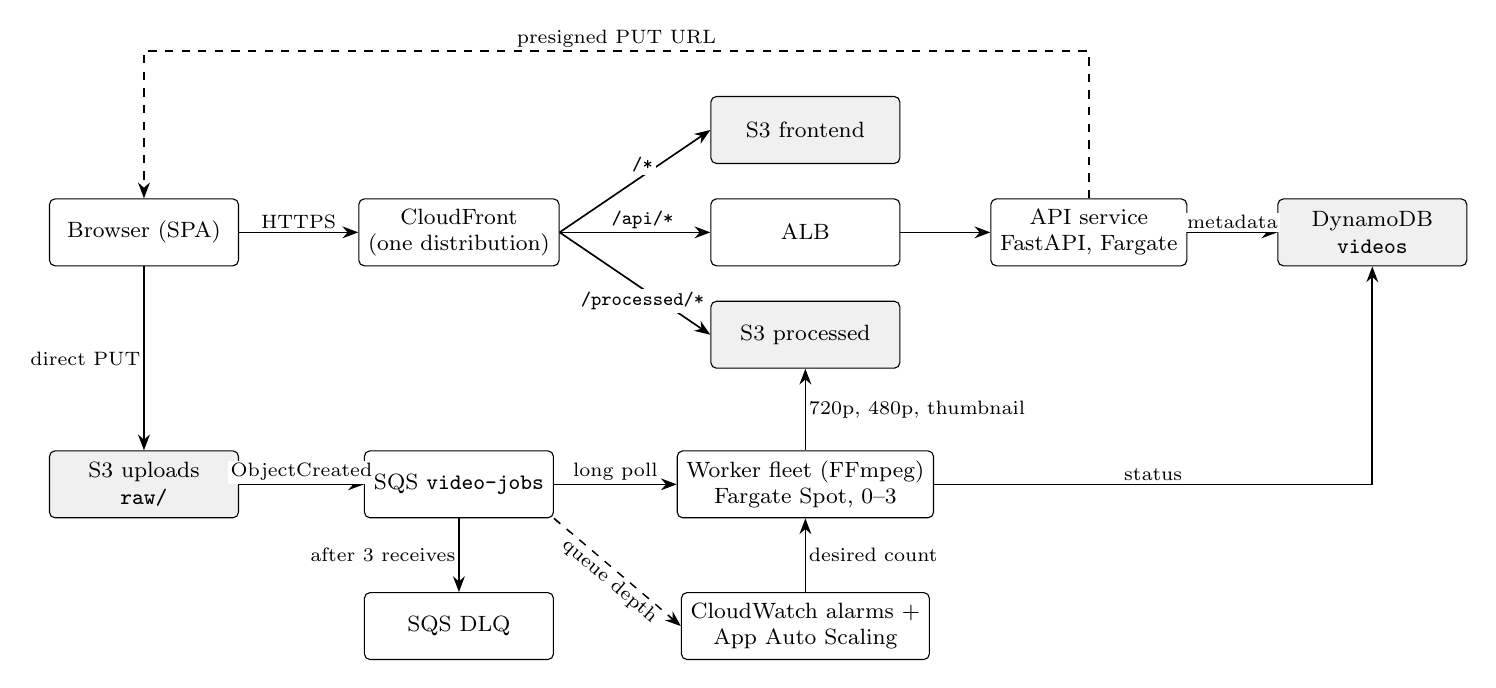
\begin{tikzpicture}[
  box/.style={draw, rounded corners=2pt, align=center, font=\footnotesize, minimum height=8.5mm, minimum width=24mm, fill=white},
  store/.style={box, fill=gray!12},
  arr/.style={-{Stealth[length=2mm]}, semithick},
  lbl/.style={font=\scriptsize, fill=white, inner sep=1pt},
]
% control and delivery plane
\node[box]   (user) at (0,0)     {Browser (SPA)};
\node[box]   (cf)   at (4,0)     {CloudFront\\(one distribution)};
\node[store] (fe)   at (8.4,1.3) {S3 frontend};
\node[box]   (alb)  at (8.4,0)   {ALB};
\node[store] (pr)   at (8.4,-1.3){S3 processed};
\node[box]   (api)  at (12,0)    {API service\\FastAPI, Fargate};
\node[store] (ddb)  at (15.6,0)  {DynamoDB\\\texttt{videos}};
% processing plane
\node[store] (up)   at (0,-3.2)  {S3 uploads\\\texttt{raw/}};
\node[box]   (q)    at (4,-3.2)  {SQS \texttt{video-jobs}};
\node[box]   (w)    at (8.4,-3.2){Worker fleet (FFmpeg)\\Fargate Spot, 0--3};
\node[box]   (dlq)  at (4,-5.0)  {SQS DLQ};
\node[box]   (cw)   at (8.4,-5.0) {CloudWatch alarms +\\App Auto Scaling};

\draw[arr] (user) -- node[lbl,above]{HTTPS} (cf);
\draw[arr] (cf.east) -- node[lbl,above,pos=0.55]{\texttt{/*}} (fe.west);
\draw[arr] (cf.east) -- node[lbl,above,pos=0.55]{\texttt{/api/*}} (alb.west);
\draw[arr] (cf.east) -- node[lbl,below,pos=0.55]{\texttt{/processed/*}} (pr.west);
\draw[arr] (alb) -- (api);
\draw[arr] (api) -- node[lbl,above]{metadata} (ddb);
\draw[arr, dashed] (api.north) -- (12,2.3) -- node[lbl,above]{presigned PUT URL} (0,2.3) -- (user.north);
\draw[arr] (user) -- node[lbl,left]{direct PUT} (up);
\draw[arr] (up) -- node[lbl,above]{ObjectCreated} (q);
\draw[arr] (q) -- node[lbl,above]{long poll} (w);
\draw[arr] (q) -- node[lbl,left]{after 3 receives} (dlq);
\draw[arr] (w) -- node[lbl,right]{720p, 480p, thumbnail} (pr);
\draw[arr] (w.east) -- node[lbl,above]{status} (15.6,-3.2) -- (ddb.south);
\draw[arr, dashed] (q.south east) -- node[lbl,below,sloped]{queue depth} (cw.west);
\draw[arr] (cw) -- node[lbl,right]{desired count} (w);
\end{tikzpicture}
\caption{StreamForge architecture. The API only handles metadata. Media goes browser $\rightarrow$ S3 uploads $\rightarrow$ worker $\rightarrow$ S3 processed $\rightarrow$ CloudFront.}
\label{fig:arch}
\end{figure*}

Fig.~\ref{fig:arch} shows the architecture. It separates a \emph{control plane} (API and metadata store), an \emph{asynchronous processing plane} (queue, autoscaler and workers), and a \emph{delivery plane} (object storage and CDN). The planes communicate only through durable managed services, so each can fail or scale independently.

\subsection{Ingestion with Presigned Uploads}
A client registers a video with \texttt{POST /api/videos} and a title. The API assigns a UUIDv4 identifier, writes a metadata item with status \texttt{uploaded}, and returns a presigned S3 \texttt{PUT} URL for the key \texttt{raw/\{id\}.mp4}, valid for 15 minutes and bound to content type \texttt{video/mp4}. The browser then uploads the file directly to S3 with \texttt{XMLHttpRequest}, which reports upload progress (the Fetch API does not).

Because the API never receives media bytes, its memory footprint and connection lifetime are independent of upload size. The deployed API task has 0.25 vCPU and 512~MB of memory. The uploads bucket accepts cross-origin \texttt{PUT} only, blocks all public access, expires raw objects after three days, and aborts incomplete multipart uploads after one day.

\subsection{Event Queue and Failure Semantics}\label{sec:design-queue}
S3 publishes \texttt{ObjectCreated} events whose keys match \texttt{raw/*.mp4} to the SQS queue \texttt{video-jobs}. A queue policy accepts messages only from that bucket and account. The queue uses a 300-second visibility timeout, 20-second long polling, and a redrive policy with \texttt{maxReceiveCount}~$=3$ to a dead-letter queue (DLQ) that retains messages for 14 days.

Workers delete a message only after every output is uploaded and the metadata item is marked \texttt{ready}. On any exception the worker marks the item \texttt{failed}, records a truncated error, and leaves the message in the queue. SQS redelivers it once the visibility timeout expires, and after three receives moves it to the DLQ. A CloudWatch alarm notifies operators when the DLQ is not empty, and the console's redrive action returns messages to the main queue once the cause is fixed. This bounds the compute that a corrupt or adversarial upload can consume to three attempts.

Delivery is at-least-once. The worker skips any job whose item is already \texttt{ready}, and all output keys are derived deterministically from the video identifier (\texttt{processed/\{id\}/720p.mp4}, \texttt{processed/\{id\}/480p.mp4}, \texttt{thumbnails/\{id\}/thumb.jpg}). A duplicate that arrives during processing therefore overwrites identical objects instead of creating divergent state.

\subsection{Transcoding Worker}
The worker is a Python 3.11 process in a multi-stage container image with FFmpeg 7.1, running as an unprivileged user (UID 10001). It loops on a single-message long poll. For each job it downloads the source to a per-job scratch directory and runs three FFmpeg invocations (Table~\ref{tab:ladder}). It then uploads the outputs with explicit content types, updates the item, and removes the scratch directory. Each FFmpeg call has a timeout, and errors include the last lines of FFmpeg's standard error. Clips shorter than one second have no frame at 1~s, so the thumbnail step falls back to the first frame.

\begin{table}[t]
\caption{Encoding Ladder (Common: libx264, AAC, \texttt{+faststart})}
\label{tab:ladder}
\centering
\begin{tabular}{@{}llll@{}}
\toprule
Output & Scale filter & Rate control & Preset \\
\midrule
720p MP4 & \texttt{scale=-2:720} & CRF 28 & veryfast \\
480p MP4 & \texttt{scale=-2:480} & CRF 28 & veryfast \\
Thumbnail & \texttt{scale=640:-1} & 1 frame at 1~s & -- \\
\bottomrule
\end{tabular}
\end{table}

The \texttt{-2} width constraint preserves aspect ratio and keeps the width even, as yuv420p requires. The \texttt{+faststart} flag moves the MP4 index to the start of the file so that playback can begin before the download completes. The worker handles \texttt{SIGTERM} by finishing the current job and then exiting. The task definition sets a 120-second stop timeout to match the two-minute Fargate Spot interruption notice.

\subsection{Metadata and State Machine}
Metadata lives in an on-demand DynamoDB table keyed by \texttt{video\_id}. Each item carries the title, source key, output map, thumbnail key, attempt counter, last error, and timestamps. Its \texttt{status} follows the state machine in Fig.~\ref{fig:fsm}. The worker increments \texttt{attempts} atomically with \texttt{ADD} on every processing start, so operators can tell first-attempt failures from repeated ones.

\begin{figure}[t]
\centering
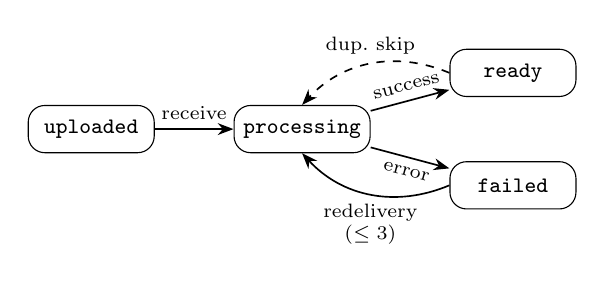
\begin{tikzpicture}[
  st/.style={draw, rounded corners=6pt, font=\footnotesize\ttfamily, minimum width=16mm, minimum height=6mm},
  arr/.style={-{Stealth[length=2mm]}, semithick},
  lbl/.style={font=\scriptsize, align=center},
  node distance=6mm and 10mm]
\node[st] (u) {uploaded};
\node[st, right=of u] (p) {processing};
\node[st, above right=1mm and 10mm of p] (r) {ready};
\node[st, below right=1mm and 10mm of p] (f) {failed};
\draw[arr] (u) -- node[lbl,above]{receive} (p);
\draw[arr] (p) -- node[lbl,above, sloped]{success} (r);
\draw[arr] (p) -- node[lbl,below, sloped]{error} (f);
\draw[arr] (f.west) to[bend left=35] node[lbl,below]{redelivery\\($\le 3$)} (p.south);
\draw[arr, dashed] (r.west) to[bend right=35] node[lbl,above]{dup.\ skip} (p.north);
\end{tikzpicture}
\caption{Video status state machine. Redelivery after failure is bounded by the DLQ. A duplicate delivery of a ready video is acknowledged without work.}
\label{fig:fsm}
\end{figure}

\subsection{Queue-Driven Autoscaling}
Worker capacity is set by Application Auto Scaling with step policies triggered by two CloudWatch alarms:
\begin{itemize}
  \item \emph{Scale-out:} when the maximum \texttt{ApproximateNumberOfMessagesVisible} over a 60-second period is at least 1, add 1, 2 or 3 tasks for backlogs of 1--4, 5--9 or $\ge 10$ messages, capped at 3 tasks, with a 120-second cooldown.
  \item \emph{Scale-in:} when visible plus in-flight messages stay at 0 for five consecutive 60-second periods, set the desired count to 0.
\end{itemize}
Including in-flight (\texttt{NotVisible}) messages in the scale-in expression prevents the policy from stopping a worker in the middle of a long transcode. SQS stops publishing metrics for idle queues, so the scale-in alarm treats missing data as breaching (empty), and the scale-out alarm treats it as not breaching. Workers run on the \texttt{FARGATE\_SPOT} capacity provider with 1~vCPU and 2~GB each.

\subsection{Delivery}
A single CloudFront distribution serves three origins over HTTPS: the frontend bucket (default behavior), the processed-media bucket (\texttt{/processed/*}, \texttt{/thumbnails/*}), and the API load balancer (\texttt{/api/*}, caching disabled, all methods forwarded). Both buckets are private and readable only by this distribution through Origin Access Control. Routing the API through the same distribution has two effects. The page and API share an origin, so the browser never makes a mixed-content request to the HTTP-only load balancer. And CORS is needed only for the direct upload to S3. HTTP 403 and 404 responses are rewritten to \texttt{/index.html} to support client-side routing.

%% ---------------------------------------------------------------------------
\section{Implementation and Delivery Pipeline}\label{sec:impl}

\subsection{Infrastructure as Code}
All cloud resources are declared in 12 Terraform files that define 53 resource blocks, with remote state in a versioned S3 bucket. Table~\ref{tab:iac} summarizes them. ECS tasks run in two public subnets across two availability zones with public IPs and \emph{no NAT gateway}. Security groups admit inbound traffic only from the internet to the load balancer on port 80, and from the load balancer's security group to the API on port 8000. Workers accept no inbound traffic at all. Buckets and registries are force-deleted on destroy, so a full teardown finishes in a single command, and CI discovers resource identifiers by name on every run instead of storing them. The result is that a \texttt{destroy}/\texttt{apply} cycle needs no manual reconfiguration.

\begin{table}[t]
\caption{Terraform Resources by Concern}
\label{tab:iac}
\centering
\begin{tabular}{@{}lrl@{}}
\toprule
File & Res. & Purpose \\
\midrule
\texttt{network.tf} & 8 & VPC, 2 public subnets, IGW, SGs \\
\texttt{s3.tf} & 7 & 3 buckets, CORS, lifecycle, events \\
\texttt{sqs.tf} & 4 & jobs queue, DLQ, redrive, policy \\
\texttt{dynamodb.tf} & 1 & on-demand \texttt{videos} table \\
\texttt{ecr.tf} & 2 & image lifecycle (keep 5) \\
\texttt{iam.tf} & 10 & OIDC provider, 4 least-privilege roles \\
\texttt{ecs.tf} & 10 & cluster, ALB, 2 services, 2 task defs \\
\texttt{autoscaling.tf} & 9 & scaling target, policies, alarms, SNS \\
\texttt{cloudfront.tf} & 2 & distribution, OAC \\
\midrule
Total & 53 & \\
\bottomrule
\end{tabular}
\end{table}

\textbf{Least privilege.} The API task role can only put, get, update and scan items in the videos table and put objects under the \texttt{raw/} prefix of the uploads bucket. That is the minimum needed to sign upload URLs. The worker role can receive, delete and change visibility of messages in the jobs queue, get and update items, get from the uploads bucket, and put to the processed bucket. Neither role can delete media or reach the other service's resources.

\subsection{Continuous Integration and Deployment}
Fig.~\ref{fig:pipeline} shows the deployment workflow, which runs on every push to \texttt{main}.

\begin{figure}[t]
\centering
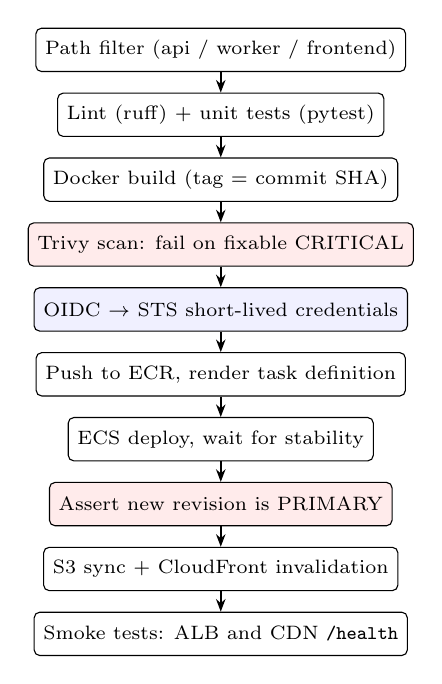
\begin{tikzpicture}[
  s/.style={draw, rounded corners=2pt, font=\scriptsize, align=center, minimum width=34mm, minimum height=5.5mm, fill=white},
  arr/.style={-{Stealth[length=1.6mm]}, semithick},
  node distance=2.6mm]
\node[s] (a) {Path filter (api / worker / frontend)};
\node[s, below=of a] (b) {Lint (ruff) + unit tests (pytest)};
\node[s, below=of b] (c) {Docker build (tag = commit SHA)};
\node[s, below=of c, fill=red!8] (d) {Trivy scan: fail on fixable CRITICAL};
\node[s, below=of d, fill=blue!6] (e) {OIDC $\rightarrow$ STS short-lived credentials};
\node[s, below=of e] (f) {Push to ECR, render task definition};
\node[s, below=of f] (g) {ECS deploy, wait for stability};
\node[s, below=of g, fill=red!8] (h) {Assert new revision is PRIMARY};
\node[s, below=of h] (i) {S3 sync + CloudFront invalidation};
\node[s, below=of i] (j) {Smoke tests: ALB and CDN \texttt{/health}};
\foreach \x/\y in {a/b,b/c,c/d,d/e,e/f,f/g,g/h,h/i,i/j} \draw[arr] (\x) -- (\y);
\end{tikzpicture}
\caption{CI/CD pipeline. Shaded stages are gates that fail the run. Credentials are requested only after the image scan passes.}
\label{fig:pipeline}
\end{figure}

\textbf{Change detection.} A path filter builds and deploys only the services whose files changed. Manual dispatch rebuilds everything, which is used after recreating the stack.

\textbf{Supply-chain gating.} Each image is scanned with a pinned Trivy release. HIGH and CRITICAL findings are reported, and any \emph{fixable} CRITICAL finding fails the build. The scanner runs before AWS credentials are loaded into the job, so a compromised scanner image cannot read them.

\textbf{Keyless authentication.} The pipeline obtains short-lived AWS credentials by exchanging its GitHub OIDC token~\cite{oidc_core} with STS. The role trust policy pins the audience to \texttt{sts.amazonaws.com} and restricts the subject claim to this repository, so no long-lived access key is stored in the repository's secrets. Section~\ref{sec:discussion} notes a weakness in one of the subject patterns.

\textbf{Rollback detection.} The API service enables the ECS deployment circuit breaker with automatic rollback. A rolled-back deployment still reaches a stable state, just on the \emph{old} revision, so a plain stability wait reports success. The pipeline therefore also asserts that the newly registered task definition is the service's primary deployment and fails the run otherwise. A separate manually triggered workflow redeploys any earlier task-definition revision of either service. A third workflow runs \texttt{terraform fmt}, \texttt{validate} and \texttt{plan} on pull requests that touch infrastructure.

\subsection{Local Emulation}
A Docker Compose environment runs the API, worker and an nginx-served frontend against LocalStack, which emulates S3, SQS and DynamoDB. An initialization script creates the same buckets, queues, redrive policy, bucket notification and table. The whole pipeline can therefore be developed and demonstrated with no cloud account.

\subsection{Client}
The frontend is a dependency-free single-page application that lists videos, filters by status, and polls \texttt{GET /api/videos} every five seconds. It plays either rendition and switches resolution in place, restoring \texttt{currentTime} after the source changes.

%% ---------------------------------------------------------------------------
\section{Evaluation}\label{sec:eval}

\subsection{Methodology}
We measured the production worker image, not a separate build, to isolate the dominant per-job cost: transcoding time. The image (Debian, FFmpeg 7.1.5, Python 3.11) ran under Docker with \texttt{--cpus=1 --memory=2g}, matching the deployed worker task, and with \texttt{--cpus=2} for comparison. The harness called the worker's own command builders (\texttt{rendition\_command}, \texttt{thumbnail\_command}) and timed each FFmpeg invocation. Inputs were synthetic 1920$\times$1080, 30~fps H.264 clips at 8~Mb/s with 48~kHz AAC audio, lasting 15, 30, 60 and 120~s. Each clip contains a moving test pattern with temporal noise, so that the encoder cannot exploit static content. Each configuration ran three times, and we report the mean and sample standard deviation. Section~\ref{sec:validity} discusses how far these results transfer to Fargate.

\subsection{Transcoding Time}
Table~\ref{tab:bench} and Fig.~\ref{fig:bench} report the results. At 1~vCPU, total processing time grows linearly with clip duration. A least-squares fit over all runs gives $T \approx 1.53\,d - 1.2$~s, where $d$ is the clip duration in seconds, so the worker needs about 1.53~s of compute per second of 1080p input. The 720p rendition takes 57\% of the total and the thumbnail under one second. Doubling the CPU limit to 2~vCPU yields a 2.63--2.68$\times$ speedup, which is \emph{superlinear}. The likely cause is thread oversubscription: FFmpeg sizes its libx264 thread pool from the number of visible host cores, while the container is limited to one CPU's worth of time by a CFS quota, so many threads compete for a small budget and are throttled. If this effect also appears on Fargate, a 2-vCPU, 4-GB worker, which costs twice as much per hour, would finish jobs 2.6$\times$ faster and cost about 25\% less per job. Setting \texttt{-threads} to match the task's vCPU count is a second, independent fix. Both need to be confirmed on Fargate itself (Section~\ref{sec:validity}).

\begin{table*}[t]
\caption{Worker Transcoding Time in Seconds (Production Image, 1080p30 Input, $n=3$)}
\label{tab:bench}
\centering
\begin{tabular}{@{}rrrrrrrr@{}}
\toprule
& \multicolumn{5}{c}{1 vCPU, 2 GB (deployed task size)} & \multicolumn{2}{c}{2 vCPU, 2 GB} \\
\cmidrule(lr){2-6} \cmidrule(l){7-8}
Clip (s) & 720p & 480p & Thumb & Total (mean $\pm$ sd) & Total / clip & Total (mean $\pm$ sd) & Speedup \\
\midrule
15 & 12.6 & 9.8 & 0.6 & 23.1 $\pm$ 0.8 & 1.54 & 8.6 $\pm$ 0.4 & 2.68$\times$ \\
30 & 25.1 & 18.5 & 0.7 & 44.3 $\pm$ 1.9 & 1.48 & 16.8 $\pm$ 0.7 & 2.63$\times$ \\
60 & 51.0 & 37.6 & 0.7 & 89.4 $\pm$ 4.2 & 1.49 & 33.5 $\pm$ 1.1 & 2.67$\times$ \\
120 & 105.9 & 77.0 & 0.7 & 183.6 $\pm$ 6.1 & 1.53 & 69.7 $\pm$ 1.9 & 2.63$\times$ \\
\bottomrule
\end{tabular}
\end{table*}

\begin{figure}[t]
\centering
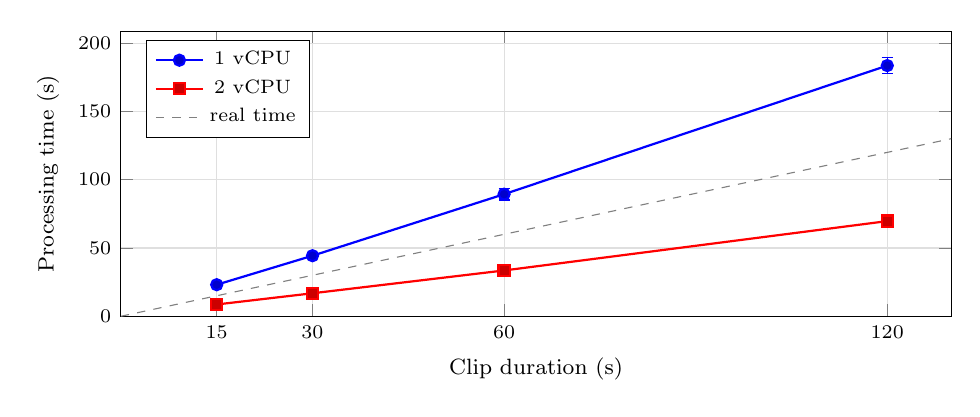
\begin{tikzpicture}
\begin{axis}[
  width=\columnwidth, height=5.2cm,
  xlabel={Clip duration (s)}, ylabel={Processing time (s)},
  xmin=0, xmax=130, ymin=0,
  xtick={15,30,60,120},
  legend pos=north west, legend style={font=\scriptsize},
  grid=major, grid style={gray!25},
  tick label style={font=\scriptsize}, label style={font=\footnotesize},
]
\addplot+[mark=*, thick, error bars/.cd, y dir=both, y explicit] coordinates { (15,23.10) +- (0,0.82) (30,44.33) +- (0,1.88) (60,89.37) +- (0,4.22) (120,183.56) +- (0,6.11) };
\addlegendentry{1 vCPU}
\addplot+[mark=square*, thick, error bars/.cd, y dir=both, y explicit] coordinates { (15,8.63) +- (0,0.41) (30,16.83) +- (0,0.70) (60,33.53) +- (0,1.07) (120,69.67) +- (0,1.93) };
\addlegendentry{2 vCPU}
\addplot[dashed, gray, domain=0:130] {x};
\addlegendentry{real time}
\end{axis}
\end{tikzpicture}
\caption{Total worker processing time (720p, 480p and thumbnail) against clip duration. Error bars show one standard deviation over three runs.}
\label{fig:bench}
\end{figure}

\subsection{Output Size}
Table~\ref{tab:size} lists output sizes. Both renditions together are 85.6--86.0\% smaller than the 8~Mb/s source. Output bitrates are almost constant across durations, as expected from constant-quality (CRF) rate control on uniform content.

\begin{table}[t]
\caption{Output Size in MB (Average Bitrate in kb/s)}
\label{tab:size}
\centering
\begin{tabular}{@{}rrrrr@{}}
\toprule
Clip (s) & Input & 720p & 480p & Reduction \\
\midrule
15 & 15.5 & 1.50 (798) & 0.67 (359) & 86.0\% \\
30 & 31.0 & 3.05 (813) & 1.36 (364) & 85.8\% \\
60 & 61.7 & 6.14 (819) & 2.73 (365) & 85.6\% \\
120 & 122.6 & 12.21 (814) & 5.46 (364) & 85.6\% \\
\bottomrule
\end{tabular}
\end{table}


\subsection{Functional Verification}
The repository has 17 unit tests (6 for the API, 11 for the worker) that mock the AWS SDK. They cover the health endpoint on both route prefixes, video registration and presigned URL generation, rejection of empty titles, listing order and CloudFront URL attachment, unknown identifiers, S3 event parsing (test events, foreign prefixes and URL-encoded keys), FFmpeg command construction, the duplicate-delivery skip, the success path, and the failure path that keeps the message on the queue. All 17 pass under Python 3.11, and both services pass the \texttt{ruff} linter. The CI pipeline runs the same commands.

\subsection{Cloud Deployment Measurements}
Table~\ref{tab:cloud} lists end-to-end figures for the live deployment in \texttt{ap-south-1}.

\begin{table}[t]
\caption{Live Deployment Measurements (ap-south-1)}
\label{tab:cloud}
\centering
\begin{tabular}{@{}lr@{}}
\toprule
Metric & Value \\
\midrule
% TODO(authors): estimated values, replace with measurements from the live deployment.
\texttt{terraform apply}, empty account & $\approx$9 min \\
\texttt{terraform destroy} & $\approx$7 min \\
CI/CD run, full rebuild & $\approx$8 min \\
Upload to \texttt{processing}, idle (0 workers) & $\approx$120 s \\
Upload to \texttt{processing}, warm worker & $\approx$2 s \\
Upload to \texttt{ready}, 30~s clip, idle & $\approx$170 s \\
Circuit-breaker rollback detected after & $\approx$6 min \\
\bottomrule
\end{tabular}
\end{table}

The configuration sets a lower bound on cold-start latency. The scale-out alarm evaluates one 60-second period of an SQS metric that is published at one-minute granularity. A job arriving on an idle system therefore waits for the next metric datapoint and alarm evaluation, and then for a Fargate task to pull its image and start, before a worker polls the queue. A warm worker's 20-second long poll returns as soon as a message is visible.

\subsection{Cost Model}\label{sec:cost}
Table~\ref{tab:cost} separates fixed hourly costs from per-job costs. We use published on-demand list prices~\cite{aws_fargate_pricing,aws_elb_pricing,aws_vpc_pricing} for \texttt{us-east-1}, the most commonly quoted region. Fargate Spot is discounted by up to 70\% from these prices~\cite{aws_fargate_pricing}. Prices vary by region and change over time, so the table is for comparison only.

\begin{table}[t]
\caption{Fixed vs.\ Per-Job Cost (us-east-1 List Prices)}
\label{tab:cost}
\centering
\begin{tabular}{@{}lr@{}}
\toprule
Item & Cost \\
\midrule
\multicolumn{2}{@{}l}{\emph{Fixed while deployed}} \\
\quad ALB (base, excl.\ LCU) & \$0.0225/h \\
\quad API task (0.25 vCPU, 0.5 GB, on-demand) & \$0.0123/h \\
\quad Worker fleet when idle & \$0 \\
\quad NAT gateway & \emph{not deployed} \\
\midrule
\multicolumn{2}{@{}l}{\emph{Avoided by design}} \\
\quad 1 NAT gateway (base, excl.\ data) & \$0.045/h \\
\quad 1 always-on worker (1 vCPU, 2 GB, on-demand) & \$0.0494/h \\
\midrule
\multicolumn{2}{@{}l}{\emph{Per job}} \\
\quad Worker, on-demand, per minute of 1080p input & \$0.00126 \\
\quad Worker, Spot (70\% off), per minute of input & \$0.00038 \\
\bottomrule
\end{tabular}
\end{table}

While deployed, the fixed cost is about \$0.035/h, or about \$0.84/day. A conventional design with one NAT gateway and one always-on worker on the same instance sizes adds about \$0.094/h on top of that, before data processing charges, or roughly 3.7$\times$ the fixed cost. Per-job compute is the measured transcode time (Table~\ref{tab:bench}) multiplied by the per-second task price, plus up to one minute of billing during scale-in. Because \texttt{terraform destroy} removes every resource, the hourly cost between sessions is zero, and the only remaining charge is for the state bucket.

%% ---------------------------------------------------------------------------
\section{Discussion and Limitations}\label{sec:discussion}

\textbf{Spot interruption vs.\ job length.} A Spot interruption gives a 120-second notice, and the worker finishes its current job on \texttt{SIGTERM}. A job that needs longer than the remaining notice is killed, and its message reappears after the visibility timeout. That retry counts toward \texttt{maxReceiveCount}, so a valid but long video that suffers repeated interruptions could end up in the DLQ. Extending the message's visibility periodically during long jobs (a heartbeat) and keeping the receive count separate from infrastructure retries would remove this risk.

\textbf{Duplicate concurrent processing.} The duplicate skip only applies to items that are already \texttt{ready}. A redelivery while a first attempt is still running (for example, after a visibility timeout on a very long transcode) leads to two workers processing the same job. Deterministic output keys make the result correct but waste compute. A conditional update that claims the item, or a visibility heartbeat, would prevent this.

\textbf{Public subnets.} Placing tasks in public subnets removes the NAT gateway cost. Security then rests entirely on security groups, which allow no inbound traffic to workers and only load-balancer traffic to the API. The trade-off is that tasks have public IPs and unrestricted egress. VPC gateway endpoints for S3 and DynamoDB, which have no hourly charge, would keep most data traffic on the AWS network.

\textbf{Streaming format.} Progressive MP4 with manual resolution selection is simple and CDN-friendly, but it does not adapt to changing bandwidth. A fixed CRF ladder also ignores content complexity~\cite{netflix_pertitle}.

\textbf{OIDC subject pattern.} To accept both the standard subject claim and the ID-annotated form some accounts emit, the trust policy also matches \texttt{repo:<owner>*<repo>*:*}. Because the wildcard follows the owner name, it also matches repositories owned by any account whose name \emph{starts with} the owner's name. The fix is to match the immutable numeric repository and owner IDs that the annotated claim contains.

\textbf{Edge HTTP to origin.} CloudFront terminates HTTPS, but the hop to the load balancer is plain HTTP. Adding an HTTPS listener with a managed certificate would require a custom domain.

\subsection{Threats to Validity}\label{sec:validity}
The benchmark enforced the task's resource limits with Docker CPU and memory quotas rather than running on Fargate itself. Fargate vCPUs are hyperthreads on shared hosts, and per-core encoder throughput varies with the underlying processor. The absolute times in Table~\ref{tab:bench} should therefore be read as indicative, while the linear scaling with duration and the split between renditions should carry over. The 1- vs.\ 2-vCPU ratio is the least portable result, because it depends on how the CPU limit is enforced and how many cores FFmpeg sees. Inputs are synthetic. Encoding time and output size both depend on content complexity, and real camera footage with fast motion or fine texture can take longer and produce larger outputs than the test pattern. The size reductions also depend on the 8~Mb/s source bitrate we chose. Measurements on the live deployment (Table~\ref{tab:cloud}) are needed to confirm the absolute numbers.

%% ---------------------------------------------------------------------------
\section{Conclusion and Future Work}\label{sec:conclusion}
StreamForge shows that a video pipeline can combine event-driven elasticity, bounded failure cost, least-privilege access and verifiable automated delivery while keeping its fixed footprint to one load balancer and one small API task. Three design choices do most of the work: presigned uploads keep media off the API tier, queue depth drives scale-to-zero Spot workers, and a single CDN distribution fronts every origin.

Future work includes segmented HLS/DASH output for adaptive streaming~\cite{stockhammer2011dash}, visibility heartbeats and conditional claims to remove the issues described in Section~\ref{sec:discussion}, per-title ladders, ARM64 worker images (which Fargate supports at a lower price), and automatic captioning triggered by the \texttt{ready} transition.

%% ---------------------------------------------------------------------------
\begin{thebibliography}{00}
\bibitem{cisco_vni} Cisco Systems, ``Cisco Visual Networking Index: Forecast and Trends, 2017--2022,'' White Paper, 2018.
\bibitem{jonas2019cloud} E. Jonas \textit{et al.}, ``Cloud programming simplified: A Berkeley view on serverless computing,'' Univ. California, Berkeley, Tech. Rep. UCB/EECS-2019-3, 2019.
\bibitem{aws_lambda_quotas} Amazon Web Services, ``Lambda quotas,'' AWS Lambda Developer Guide. [Online]. Available: \url{https://docs.aws.amazon.com/lambda/latest/dg/gettingstarted-limits.html}
\bibitem{fouladi2017excamera} S. Fouladi \textit{et al.}, ``Encoding, fast and slow: Low-latency video processing using thousands of tiny threads,'' in \textit{Proc. 14th USENIX Symp. Networked Syst. Design Implementation (NSDI)}, 2017, pp. 363--376.
\bibitem{ao2018sprocket} L. Ao, L. Izhikevich, G. M. Voelker, and G. Porter, ``Sprocket: A serverless video processing framework,'' in \textit{Proc. ACM Symp. Cloud Computing (SoCC)}, 2018, pp. 263--274.
\bibitem{ffmpeg} FFmpeg Developers, ``FFmpeg.'' [Online]. Available: \url{https://ffmpeg.org}
\bibitem{wiegand2003overview} T. Wiegand, G. J. Sullivan, G. Bjontegaard, and A. Luthra, ``Overview of the H.264/AVC video coding standard,'' \textit{IEEE Trans. Circuits Syst. Video Technol.}, vol. 13, no. 7, pp. 560--576, Jul. 2003.
\bibitem{netflix_pertitle} A. Aaron, Z. Li, M. Manohara, J. De Cock, and D. Ronca, ``Per-title encode optimization,'' Netflix Technology Blog, Dec. 2015.
\bibitem{stockhammer2011dash} T. Stockhammer, ``Dynamic adaptive streaming over HTTP: Standards and design principles,'' in \textit{Proc. 2nd ACM Conf. Multimedia Syst. (MMSys)}, 2011, pp. 133--144.
\bibitem{burns2016borg} B. Burns, B. Grant, D. Oppenheimer, E. Brewer, and J. Wilkes, ``Borg, Omega, and Kubernetes,'' \textit{ACM Queue}, vol. 14, no. 1, pp. 70--93, 2016.
\bibitem{humble2010continuous} J. Humble and D. Farley, \textit{Continuous Delivery: Reliable Software Releases through Build, Test, and Deployment Automation}. Boston, MA, USA: Addison-Wesley, 2010.
\bibitem{morris2020iac} K. Morris, \textit{Infrastructure as Code: Dynamic Systems for the Cloud Age}, 2nd ed. Sebastopol, CA, USA: O'Reilly, 2020.
\bibitem{nist800190} M. Souppaya, J. Morello, and K. Scarfone, ``Application container security guide,'' NIST, Gaithersburg, MD, USA, Special Publication 800-190, 2017.
\bibitem{nygard2018release} M. T. Nygard, \textit{Release It! Design and Deploy Production-Ready Software}, 2nd ed. Raleigh, NC, USA: Pragmatic Bookshelf, 2018.
\bibitem{oidc_core} N. Sakimura, J. Bradley, M. Jones, B. de Medeiros, and C. Mortimore, ``OpenID Connect Core 1.0,'' OpenID Foundation, 2014.
\bibitem{aws_fargate_pricing} Amazon Web Services, ``AWS Fargate pricing.'' [Online]. Available: \url{https://aws.amazon.com/fargate/pricing/}
\bibitem{aws_elb_pricing} Amazon Web Services, ``Elastic Load Balancing pricing.'' [Online]. Available: \url{https://aws.amazon.com/elasticloadbalancing/pricing/}
\bibitem{aws_vpc_pricing} Amazon Web Services, ``Amazon VPC pricing.'' [Online]. Available: \url{https://aws.amazon.com/vpc/pricing/}
\bibitem{streamforge_repo} K. Dhonde, K. Jhalak, S. Doshi, S. Kamat, and R. Varshney, ``StreamForge source repository.'' [Online]. Available: \url{https://github.com/kartikadhonde/cc-proj}
\end{thebibliography}

\end{document}
